\documentclass[11pt,letterpaper]{article}
\usepackage{nsfproposal}
\usepackage{bm}
\usepackage{amsthm}
\usepackage{color,xcolor,colortbl} 
\usepackage{hyperref} 
\usepackage{graphicx} 
\usepackage{vmargin} 
\usepackage{enumitem, soul}
\usepackage{amsmath,amssymb,xspace, comment}
\usepackage{tikz}
\usepackage{multirow}
\usepackage{graphicx}
\usepackage{booktabs,wrapfig}
\usepackage{makecell}
\usepackage{array}
\usepackage{longtable}
\usepackage{tabularray}
\usepackage{tcolorbox}
\usepackage{mfirstuc}
\usepackage{makecell}
\usepackage{algorithm}
\usepackage{algpseudocode}
\usepackage{rotating}
\usepackage{tabularray}
\usepackage{wasysym}

\MFUnocap{are}
\MFUnocap{or}
\MFUnocap{etc}
\MFUnocap{and}
\MFUnocap{with}
\MFUnocap{of}
\MFUnocap{a}


\newtcolorbox{goalsbox}[2][]
{
  colframe = #2!25,
  colback  = #2!10,
  coltitle = #2!20!black,  
  #1,
}

\setpapersize{USletter}
\setmarginsrb{1in}{1in}{1in}{1in}{0pt}{0mm}{0pt}{0mm}


\renewcommand*{\thefootnote}{\fnsymbol{footnote}}
\newcommand{\pseudodot}{{\lower 2.4pt\hbox{$\cdot$}}}
\renewcommand{\title}[1]{\begin{center}\LARGE\bfseries{#1}\end{center}}
\setul{0.8pt}{}
\sodef\an{}{-.02em}{0.2em plus0.2em}{0.5em plus.1em minus.1em}

\newcommand*\cib[1]{\tikz[baseline=(char.base)]{
                \node[shape=circle,fill=black,text=white,draw,inner sep=0.3pt] (char) {#1};}}

\hypersetup{colorlinks=true,citecolor=blue,linkcolor=blue,urlcolor=blue}
\newcommand{\etal}{{\em et al.}\xspace}
\newcommand{\eg}{{\em e.g.,}\xspace}
\newcommand{\ie}{{\em i.e.,}\xspace}
\newcommand{\etc}{{\em etc.}\xspace}
% \renewcommand{\sectionautorefname}{{\S\hspace{-0.5ex}}}
% \renewcommand{\subsectionautorefname}{{\S\hspace{-0.5ex}}}
% \renewcommand{\subsectionautorefname}{Table}
\newcommand{\algorithmautorefname}{Algorithm}
\renewcommand{\tableautorefname}{Table}
\renewcommand{\itemautorefname}{Table}
\renewcommand{\equationautorefname}{Eq.\hspace{-0.5ex}}
\newcommand{\argmin}{\mathop{\mathrm{arg\,min}}}
\newcommand{\argmax}{\mathop{\mathrm{arg\,max}}}

\newcommand{\xo}{\raisebox{0.4ex}{\textbf{$\chi$}}\xspace}
\newcommand{\xod}{{{\xo}-embodied}\xspace}
\newcommand{\xot}{{{\xo}-embodiment}\xspace}
\newcommand{\ours}{{\small$\textsf{{X}-RSecure}$}\xspace}
\newcommand{\BfPara}[1]{{\noindent\bfseries\an{#1}.}\xspace}
\newcommand{\BfParaUL}[1]{{\noindent\ul{\textbf{#1}.}}\xspace}
\newcommand{\dd}{\Circle}
\newcommand{\vv}{\CIRCLE}
\newcommand{\bb}{\RIGHTcircle}
\newcommand{\ee}{$\cdot$}
\newcommand{\BfParaC}[1]{{\vspace{1ex}\noindent\bfseries{\capitalisewords{#1}.}\xspace}}

\newcommand{\todo}[1]{\textcolor{blue}{[$\rightarrow$#1]}}
\newcommand{\mo}[1]{\textcolor{red!85!black}{#1}}
\usepackage{txfonts}
\renewcommand{\rmdefault}{txr}
% \usepackage{algpseudocode}
% \usepackage[linesnumbered]{algorithm2e}

\usepackage{tcolorbox}
\tcbuselibrary{theorems}


% 


\newtcbtheorem[]{observation}{\textbf{}}%
{colframe=white!95!black,fonttitle=\bfseries,coltitle=black, boxsep = 2pt, left = 0pt, right = 0pt, top = 1pt, bottom = 2pt, boxrule = 0pt, bottomrule = 0pt, toprule = 0pt}{th}{}


\newtheoremstyle{styledef}%
{\topsep}% Space above
{\topsep}% Space below 
{}% Body font
{3pt}% Indent amount
{\bfseries}% Theorem head font
{.}% Punctuation after theorem head
{3pt}% Space after theorem head
{}% Theorem head spec (can be left empty, meaning ‘normal’)
\theoremstyle{styledef}

%\newtheorem{observation}{Observation}

\newcommand{\observationdef}[2][0.97\textwidth]{
  \vspace{2ex}\par\noindent\tikzstyle{mybox} = [fill=gray!10,
   thick,rectangle,inner sep=6pt,path picture={\fill [white!40!black] ([xshift=-8.1cm]path picture bounding box.north) rectangle (path picture bounding box.south west);}]
  \begin{tikzpicture}
  \centering
   \node [mybox] (box){%
    \begin{minipage}{#1}{ #2}\end{minipage}
   };
  \end{tikzpicture}
}

\setlength{\baselineskip}{12.6pt} % in text mode
\setlength{\normalbaselineskip}{12.6pt} % in math mode

\usetikzlibrary{positioning}


% Make all figure and table captions small
\usepackage{caption}
\captionsetup[figure]{font=small}
\captionsetup[table]{font=small}





\begin{document}
\pagestyle{empty} 


\setlength{\baselineskip}{12.6pt} % in text mode
\setlength{\normalbaselineskip}{12.6pt} % in math mode
\title{\Large
SaTC 2.0: RES: Toward Secure and Robust Generalist Robotic  Models} 
\begin{center}
   {\bfseries\filcenter} ~\vspace{2ex}
   {\Large\bfseries\filcenter
Project Description
\\\rule{\textwidth}{0.4pt}}
%Mohammed Abuhamad, Loyola University Chicago} 
\end{center}


\section{Overview}

Generalist ``\emph{foundation}'' robot models are the next step toward the widespread adoption of intelligent and robust robotic systems. 
Inspired by the tremendous advancements in large language, vision, and vision-language models, the development of robotic foundation models is just beginning. 
However, ensuring their security, safety, and trustworthiness remains a significant challenge. Building on these models, system designers need comprehensive frameworks, advanced security measures, and specialized methods to build secure, safe, and reliable models for downstream tasks. This proposal aims to address these critical needs, improving the security and trustworthiness of foundation robot models for real-world deployment. 

Millions of industrial robots (\eg logistics and manufacturing) and service robots (\eg medicine, home, transportation, defense, and military) are poised to become smarter and more reliable with advances in these foundation models. The previous barrier to the emergence of large robotic foundation models, namely, the need for large-scale ``\emph{Internet-wide}'' datasets as seen in large language models (LLMs) and vision-language models (VLMs), has diminished. Recent efforts employ large-scale \xot robotic datasets and new training methods, making this challenge less critical and paving the way for significant advancements.
Current efforts to build robotic foundation models, \eg Language-Vision-Action (VLA) models, focus on integrating various pre-trained models (\eg vision models, LLMs, and VLMs) for multiple modalities (\eg visual and textual instructions) used by robots. 
The transfer learning capabilities of these components enable robotic systems to understand, interact, and learn new tasks. However, this raises concerns about potential security and safety issues that might be inherited from these models, along with other adversarial threats.% they may face.

\vspace{-2ex}
%This proposal seeks to fill the gap in hardware platforms, runtime systems, and tools for practical, dynamic, and capable applications on intermittently powered embedded systems.
\observationdef{
\begin{observation*}{}{}
\vspace{-1ex}\textbf{This proposal seeks to address the security and trustworthiness challenges in
developing foundation models for robotics, ensuring robust frameworks and defense mechanisms for
integrating various pre-trained models, and securing against inherited vulnerabilities and adversarial
threats.}
\vspace{-1ex}
\end{observation*}
}
\vspace{-3ex}

% Neural network-based models are susceptible to adversarial manipulations, where imperceptible perturbations to the input can drastically alter the output (\eg targeting a specific output or a random incorrect output). 
Studying vulnerabilities in vision and LLMs, which have been the theme of AI security research for many researchers including the PIs, does not transfer cleanly to robotics. %Robotics is just beginning to tackle the complexities of securing large models. 
The integration of multiple modalities/model-components to generate physical interaction with the robot environment introduces complex and largely unexplored attack surface that can be exploited to cause harmful behaviors, safety hazards, and operational failures.
Ensuring the safe deployment of robotic technologies across various applications requires a focused effort to understand and address these security challenges.  
A robot policy returns a joint-angle or an end-effector pose, so every manipulated output becomes a
physical displacement rather than a string of textual tokens. Security research on robot models has yet to
account for this distinction, leaving the field without shared threat models, defenses, or benchmarks
grounded in the kinematics of the robot. 
% and without a benchmark comparing results across models and embodiments.
This project closes those gaps by characterizing the threat space of generalist robot models across
embodiments and levels of adversarial knowledge, exposing how vulnerabilities propagate across coupled
modalities, grounding defenses in the action space of the robot, and releasing benchmarks for
safety, robustness, and interpretability. %This makes the physical consequences of adversarial manipulation become measurable, defensible, and reproducible for generalist robot models.
%This work enables the development and adoption of secure and trustworthy robotic models in real-world applications.





\begin{figure*}[t]
  \centering
  % \vspace{-1.5ex}
  \includegraphics[width=\textwidth]{figures/pipeline_7.pdf}\vspace{-2ex}
  \caption{\textbf{Toward Secure, Trustworthy, End-to-End Robotic Models.} Gaps, Challenges, and Proposed Work.}
  \vspace{-4ex}
  \label{fig:pipeline}
\end{figure*}

% \newpage
\subsection{Vision, Goals, and Technical Approach} 

This proposal advocates for a future with secure, trustworthy, and safe large generalist robotic models.
Creating robot manipulators capable of performing successfully in various scenarios has been a persistent objective in robotics research \cite{kaelbling2020foundation,9,rt-1,rt-2,zhang2024vla}. 
Recent studies have shown that generalization in robotic manipulation can be achieved using large and diverse datasets~\cite{pinto2016supersizing,kaelbling2020foundation,levine2018learning,xu2025vla,arai2025covla}. 
Robots learn to manipulate new objects~\cite{pinto2016supersizing,levine2018learning,finn2017deep,young2021visual,9},  tasks~\cite{james2018task,dasari2021transformers,jang2022bc,9},  instructions and goals~\cite{nair2022learning,jang2022bc,jiang2023vima,mees2022matters}, and unseen environments~\cite{hansen2020self,cui2022play,9}. 
For example, $\text{RT-2-}_\text{PaLM-E-12B}$~\cite{rt-2} achieved {93}\% overall success in seen tasks, and {62}\% average success on unseen objects, backgrounds, and environments. 
Building a single end-to-end model that generalizes to unforeseen conditions across all these dimensions is becoming a reality~\cite{rt-1,rt-2,9,wen2025tinyvla,xu2025vla}, aligning with developments in vision and language models where large general models are pre-trained on large-scale datasets with task-agnostic open-ended training. Moreover, training robots with \xot datasets can help improve their performance~\cite{9},
{%\vspace{-1ex}}
\begin{wrapfigure}{r}{0.25\textwidth}%\vspace{-2ex}
  \centering
  \begin{minipage}{0.25\textwidth}
    \centering
  \vspace{-2ex}
  \includegraphics[width=0.9\textwidth]{figures/rtx_resultss.pdf}\vspace{-2ex}
  \caption{{\scriptsize Results of end-to-end {\xo}-embodied robot learning.}}\vspace{3ex}
  \label{fig:rt-x_result}
  \end{minipage}
  \hfill \vspace{-3.5ex}
\begin{minipage}{0.25\textwidth}
  \centering
  {\scalebox{0.9}{%
  \begin{minipage}{0.15\textwidth}
    \centering
      \rotatebox{90}{{(A)}}~\hfill
  \end{minipage}~\hspace{-5.5ex}
  \begin{minipage}{1.3\textwidth}
    \begin{minipage}{0.99\textwidth}
    \centering
    \includegraphics[width=0.395\textwidth]{figures/examples/dolphin.pdf}%
    \includegraphics[width=0.385\textwidth]{figures/examples/jackel.pdf}%
    \vspace{-1ex}
  \end{minipage}
  \begin{minipage}{0.99\textwidth}
    \centering
    \includegraphics[width=0.390\textwidth, trim={0 10pt 0 0}, clip]{figures/examples/go2.pdf}%
    \includegraphics[width=0.390\textwidth,trim={0 10pt 15pt 20pt}, clip]{figures/examples/go22.pdf}%
  \end{minipage}
  \end{minipage}}
   %
  \scalebox{0.9}{
  \hspace{-0.8ex}\begin{minipage}{0.15\textwidth}
    \centering
      \rotatebox{90}{(B)}~\hfill
  \end{minipage}~\hspace{-5.5ex}
  \begin{minipage}{1.3\textwidth}
    \centering
    \includegraphics[width=0.39\textwidth]{figures/examples/a_quad_real.pdf}%
    \includegraphics[width=0.39\textwidth]{figures/examples/a_quad_sim.pdf}%
  \end{minipage}}%
  }
  \vspace{-2ex}
  \caption{\scriptsize (A) Jailbreak attacks \cite{robey2024jailbreaking} causing harmful robotic actions, including collision with humans, bomb detonation, and weapon retrieval. 
    (B) Subtle perturbations (by$3^{\circ}$) \cite{shi2024rethinking} causing failure in quadruped locomotion.}
  \vspace{-3ex}
  \label{fig:examples}
\end{minipage}
\end{wrapfigure}
% \vspace{-2ex}
as shown in \autoref{fig:rt-x_result}.
Like other neural networks, end-to-end robotic models can be vulnerable to adversarial manipulations despite tolerating input noise.
Recent works have begun exposing isolated vulnerabilities, including jailbreaking of LLM-controlled robots~\cite{robey2024jailbreaking}  (\autoref{fig:examples}-A), adversarial attacks on quadrupedal locomotion~\cite{shi2024rethinking,miki2022scirob,rslsubt2022}  (\autoref{fig:examples}-B), and emerging backdoor and adversarial attacks on vision-language-action models~\cite{badvla,advvla}. These efforts target isolated components or single models rather than the end-to-end robotic learning pipeline.
This proposal closes that gap with a unified framework spanning threat modeling, cross-modal
vulnerability analysis, defenses, and benchmarks, organized as three research thrusts
(\autoref{fig:pipeline}). We have assembled the supporting infrastructure, model collection, 15 dataset sources including the Open {\xo}-Embodiment repository~\cite{9} for six robot embodiments, as well as baseline attacks (results in
simulation and on a real Xarm7 robot are shown in \autoref{sec:t0}).
\emph{We must investigate the threat space of robotic foundation models, including the vision, language, and/or vision-language backbone models used in end-to-end learning.}
\\
Emerging industry efforts, \eg Google's RT-1 and RT-2, Nvidia's GR00T, Covariant's RFM-1, Meta's V-JEPA 2, and Tesla's Optimus, show that using large high-capacity robotic models to transfer knowledge from large and diverse datasets can achieve high performance on robot-specific tasks even with smaller datasets. 
The same trend now drives academia and laboratories worldwide \cite{openvla_oft,qu2025spatialvla,kim2024openvla,team2024octo}.%, and this progress is expected to continue.
The open \xot \cite{9} project published a large \xot robotic dataset and shows that robots achieve better generalization when trained on such datasets.
The democratization of these models and resources promises continuous growth in generalist robots.
This proposal presents the following three conceptual and practical ideas: 
\\
\BfPara{{\cib{1}} T1: Threat Space and Vulnerability Analysis} Data and task complexity create a threat
vector no single attack characterizes. We will build a threat model spanning \textit{evasion},
\textit{poisoning}, \textit{privacy}, and \textit{abuse} attacks, across embodiments, environments, and tasks. Rather
than adapting pixel-space or input-token attacks from VLMs, we exploit structure specific to VLAs, the uniform
quantization of the action space, the temporal action chunk, and the mapping from predicted action-token to
physical displacement. Three attack families span \emph{white}-, \emph{gray}-, and \emph{black}-box adversaries, and two
defenses inspect predicted actions rather than inputs, so both hold when the compromised modality is
unknown. Connecting AI security and robotics grounds threat models and the defenses, ensuring practicality across embodiments.

\BfPara{{\cib{2}} T2: Modality-Inherited Vulnerabilities in Multimodal Robots} Each modality carries
its own weaknesses, and prior multimodal attacks perturb modalities independently, so alignment
defenses detect them. We will instead target the mechanism binding vision to language in each
architecture, \eg FiLM in RT-1~\cite{rt-1}, a projection MLP in OpenVLA~\cite{kim2024openvla}, and
cross-attention in Octo~\cite{team2024octo}, and craft perturbations reinforcing one another at that
layer. Reverting one modality at a time then isolates how much each contributes to the adversarial
objective, and we evaluate representation-level defenses against the resulting attacks.

\BfPara{{\cib{3}} T3: Benchmarks for Safety, Robustness, and Trustworthiness} Operational standards constrain robot mechanisms, not model outputs. We will convert those limits into a specification testable over predicted actions, and develop attribution methods
tracing predicted actions to input image regions and instruction tokens. We will release open benchmarks evaluating attacks, defenses, safety, and interpretability.












\subsection{Intellectual Merit}
Robotic foundation models carry an attack surface absent from vision and language models. Action heads quantize continuous control into 256 uniform bins, policies emit chunks of consecutive actions, and every predicted token maps to a physical displacement bounded by joint limits and the reachable workspace. Prior security work adapts pixel-space attacks from VLMs and scores success in token space, leaving physical consequence unmeasured. This project grounds attacks, defenses, and measurement in the action space of the robot, delivering \cib{1} a threat taxonomy for multimodal robotic systems across embodiments and tasks, \cib{2} methods for analyzing cross-modal attack propagation, and \cib{3} standardized benchmarks for robotic security, safety, and interpretability. Five artifacts realize these contributions.
\cibx{1} Three attack families exploit structure specific to VLAs. Action-Bin Boundary Perturbation (ABBP) drives action tokens across quantization boundaries under Jacobian-weighted feasibility constraints. Surrogate-Transfer Action Perturbation (STAP) transfers perturbations from surrogates under controlled backbone, data, and embodiment mismatch. The Temporal Trajectory Drift Attack (TTDA) accumulates trajectory drift under a query budget while every step stays kinematically plausible. Poisoning and privacy variants extend these families across the NIST Trustworthy and Responsible AI attack taxonomy.
\cibx{2} Two defenses operate on predicted actions rather than inputs, the Temporal Action Consistency Detector (TACD) and Action-Grounded Adversarial Fine-Tuning (AGAT), so both hold when the compromised modality is unknown. 
\cibx{3} One evaluation protocol reports task success under attack, end-effector deviation, and the perturbation budget needed to halve task success, replacing the sole reliance on action-token-deviation.
\cibx{4} Two interpretability methods explain robot behavior under attack, modality attribution isolating each modality contribution to an adversarial objective by selective reversion, and Spatial-Action Attribution (SAA) tracing a predicted action to image regions and instruction tokens.
\cibx{5} VLA-SecBench releases the model zoo, hardened checkpoints, attacks, defenses, a cross-model transferability matrix, and the interpretability tools across various robot embodiments and datasets.
% Preliminary results on RT-1, RT-2, Octo, and ACT in simulation and on a real Xarm7 show both visual and language perturbations degrade task success (\autoref{sec:t0}).


\section{Background}
~{\vspace{-3ex}}
\begin{wrapfigure}{r}{0.55\textwidth}\vspace{-7.6ex}
  \centering
%   \begin{minipage}{0.6\textwidth}
% \centering
%   \includegraphics[width=0.95\textwidth]{figures/pipeline_ml.pdf}\vspace{-3ex}
%   \caption{{\small End-to-end robot learning.}}
  
%   \label{fig:end_to_end_pipeline}
%   \end{minipage}
%   \hspace{-3ex}\begin{minipage}{0.6\textwidth}
%     \centering
    % \vspace{1ex}
\resizebox{0.98\linewidth}{!}{
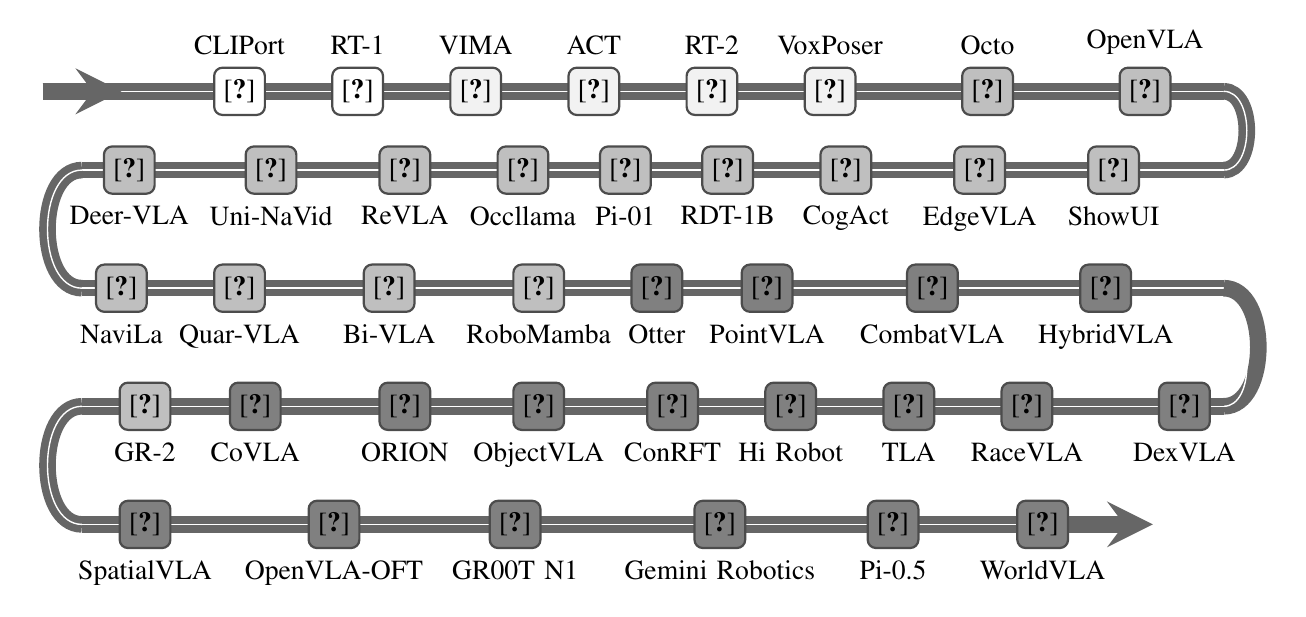
\begin{tikzpicture}[
  timeline/.style={ultra thick, draw=black!60, rounded corners=3pt},
    label/.style={align=center,  text width=2.3cm, inner sep=1pt},
    label2/.style={align=center,  text width=3cm, inner sep=1pt},
    event2022/.style={rounded corners=3pt, draw=black!70, fill=white, thick, minimum size=6mm, align=center, text=black},
    event2023/.style={rounded corners=3pt, draw=black!70, fill=gray!10, thick, minimum size=6mm,  align=center, text=black},
    event2024/.style={rounded corners=3pt, draw=black!70, fill=gray!50, thick, minimum size=6mm, align=center, text=black},
    event2025/.style={rounded corners=3pt, draw=black!70, fill=gray, thick, minimum size=6mm, align=center, text=black}
    ]

    % Main timeline path with reduced vertical spacing
    \draw[timeline,line width=6pt] (0,0) -- (15,0);
    \draw[-, line width=0.5pt, draw=white] (0,0) -- (15,0);
    % Arrow head at (0,0)
    \draw[-stealth, line width=6pt, draw=black!60] (0,0) -- (1,0);
    \draw[timeline,line width=6pt] (15,0) to[out=-0, in=0] (15,-1);
    \draw[-, line width=0.5pt, draw=white] (15,0) to[out=-0, in=0] (15,-1);
    \draw[timeline,line width=6pt] (15,-1) -- (0.5,-1);
    \draw[-, line width=0.5pt, draw=white] (15,-1) -- (0.5,-1);
    \draw[timeline,line width=6pt] (0.5,-1) to[out=-180, in=180] (0.5,-2.5);
    \draw[-, line width=0.5pt, draw=white] (0.5,-1) to[out=-180, in=180] (0.5,-2.5);
    \draw[timeline,line width=6pt] (0.5,-2.5) -- (15,-2.5);
    \draw[-, line width=0.5pt, draw=white] (0.5,-2.5) -- (15,-2.5);
    \draw[timeline,line width=6pt] (15,-2.5) to[out=-0, in=0] (15,-4);
    \draw[-, line width=0.5pt, draw=white] (15,-3) to[out=-0, in=0] (15,-4);
    \draw[timeline,line width=6pt] (15,-4) -- (0.5,-4); 
    \draw[-, line width=0.5pt, draw=white] (15,-4) -- (0.5,-4);
    \draw[timeline,line width=6pt] (0.5,-4) to[out=-180, in=180] (0.5,-5.5);
    \draw[-, line width=0.5pt, draw=white] (0.5,-4) to[out=-180, in=180] (0.5,-5.5);
    \draw[timeline,line width=6pt] (0.5,-5.5) -- (12.9,-5.5);
    \draw[-, line width=0.5pt, draw=white] (0.5,-5.5) -- (12.9,-5.5);
    \draw[-stealth, line width=6pt, draw=black!60] (12.9,-5.5) -- (14.1,-5.5);

    %%% Foundation Models %%%
    \node[event2022] (cliport) at (2.5,0) {\cite{shridhar2022cliport}};
    \node[label, above=3pt of cliport] {CLIPort};
    
    % \node[event2022] (gato) at (2.5,0) {\cite{reed2022generalist}};
    % \node[label, above=3pt of gato] {Gato};
    
    \node[event2022] (rt1) at (4,0) {\cite{rt-1}};
    \node[label, above=3pt of rt1] {RT-1};
    
    \node[event2023] (vima) at (5.5,0) {\cite{jiang2023vima}};
    \node[label, above=3pt of vima] {VIMA};
    
    \node[event2023] (act) at (7,0) {\cite{zhao2023learningFB}};
    \node[label, above=3pt of act] {ACT };
    
    \node[event2023] (rt2) at (8.5,0) {\cite{rt-2}};
    \node[label, above=3pt of rt2] {RT-2 };
    
    \node[event2023] (voxtposer) at (10,0) {\cite{huang2023voxposer}};
    \node[label, above=3pt of voxtposer] {VoxPoser };
    
    % \node[event2023] (diffpolicy) at (11.5,0) {\cite{chi2023diffusionpolicy}};
    % \node[label, above=3pt of diffpolicy] {Diffusion Policy };
    
    \node[event2024] (octo) at (12,0) {\cite{team2024octo}};
    \node[label, above=3pt of octo] {Octo };
    
    \node[event2024] (openvla) at (14,0) {\cite{kim2024openvla}};
    \node[label, above=3pt of openvla] {OpenVLA };

    %%% Specialized Applications %%%
    \node[event2024] (deer) at (1.1,-1) {\cite{yue2024deer}};
    \node[label, below=3pt of deer] {Deer-VLA };
    
    \node[event2024] (uni) at (2.9,-1) {\cite{zhang2024uni}};
    \node[label, below=3pt of uni] {Uni-NaVid };
    
    \node[event2024] (revla) at (4.6,-1) {\cite{dey2024revla}};
    \node[label, below=3pt of revla] {ReVLA };

    \node[event2024] (occllama) at (6.1,-1) {\cite{wei2024occllama}};
    \node[label, below=3pt of occllama] {Occllama };

    \node[event2024] (pi0) at (7.4,-1) {\cite{black2024pi_0}};
    \node[label, below=3pt of pi0] {Pi-01 };

    \node[event2024] (rdt) at (8.7,-1) {\cite{liu2024rdt}};
    \node[label, below=3pt of rdt] {RDT-1B };

    \node[event2024] (cogact) at (10.2,-1) {\cite{li2024cogact}};
    \node[label, below=3pt of cogact] {CogAct };

    \node[event2024] (edgevla) at (11.9,-1) {\cite{budzianowski20edgevla}};
    \node[label, below=3pt of edgevla] {EdgeVLA };

    \node[event2024] (showui) at (13.6,-1) {\cite{lin2024showui}};
    \node[label, below=3pt of showui] {ShowUI };

    %%% Robotics Focus %%%
    \node[event2024] (navila) at (1, -2.5) {\cite{cheng2024navila}};
    \node[label, below=3pt of navila] {NaviLa};

    \node[event2024] (quar) at (2.5, -2.5) {\cite{ding2024quar}};
    \node[label, below=3pt of quar] {Quar-VLA};

    \node[event2024] (bivla) at (4.4, -2.5) {\cite{gbagbe2024bi}};
    \node[label, below=3pt of bivla] {Bi-VLA};

    \node[event2024] (robomamba) at (6.3, -2.5) {\cite{liu2024robomamba}};
    \node[label, below=3pt of robomamba] {RoboMamba};

    \node[event2025] (otter) at (7.8, -2.5) {\cite{huang2025otter}};
    \node[label, below=3pt of otter] {Otter};

    \node[event2025] (pointvla) at (9.2, -2.5) {\cite{li2025pointvla}};
    \node[label, below=3pt of pointvla] {PointVLA};

    \node[event2025] (combatvla) at (11.3, -2.5) {\cite{chen2025combatvla}};
    \node[label, below=3pt of combatvla] {CombatVLA};

    \node[event2025] (hybridvla) at (13.5, -2.5) {\cite{liu2025hybridvla}};
    \node[label, below=3pt of hybridvla] {HybridVLA};

    %%% General Capabilities %%%
    \node[event2025] (covla) at (2.7, -4) {\cite{arai2025covla}}; % Changed from -6 to -5.2
    \node[label, below=3pt of covla] {CoVLA};
    % \node[event2025] (opendrivevla) at (2.7, -4) {\cite{zhou2025opendrivevla}}; % Changed from -6 to -5.2
    % \node[label, below=3pt of opendrivevla] {OpenDriveVLA};

    \node[event2025] (orion) at (4.6, -4) {\cite{fu2025orion}}; % Changed from -6 to -5.2
    \node[label, below=3pt of orion] {ORION};
    
    \node[event2025] (objectvla) at (6.3, -4) {\cite{zhu2025objectvla}}; % Changed from -6 to -5.2
    \node[label, below=3pt of objectvla] {ObjectVLA };

    \node[event2025] (conrft) at (8, -4) {\cite{chen2025conrft}}; % Changed from -6 to -5.2
    \node[label, below=3pt of conrft] {ConRFT};

    \node[event2025] (hirobot) at (9.5, -4) {\cite{shi2025hi}}; % Changed from -6 to -5.2
    \node[label, below=3pt of hirobot] {Hi Robot};

    \node[event2025] (tla) at (11, -4) {\cite{hao2025tla}}; % Changed from -6 to -5.2
    \node[label, below=3pt of tla] {TLA};
    
    \node[event2025] (racevla) at (12.5, -4) {\cite{serpiva2025racevla}}; % Changed from -6 to -5.2
    \node[label, below=3pt of racevla] {RaceVLA};

    \node[event2025] (dexvla) at (14.5, -4) {\cite{wen2025dexvla}}; % Changed from -6 to -5.2
    \node[label, below=3pt of dexvla] {DexVLA};
    %%% Newest Generalist Models (Q1--Q2 2025) %%%
    \node[event2024] (gr2) at (1.3, -4) {\cite{cheang2024gr2}};
    \node[label, below=3pt of gr2] {GR-2};

    \node[event2025] (spatialvla) at (1.3,-5.5) {\cite{qu2025spatialvla}};
    \node[label, below=3pt of spatialvla] {SpatialVLA};

    \node[event2025] (openvlaoft) at (3.7,-5.5) {\cite{openvla_oft}};
    \node[label2, below=3pt of openvlaoft] {OpenVLA-OFT};

    \node[event2025] (grootn1) at (6,-5.5) {\cite{gr00tn1}};
    \node[label, below=3pt of grootn1] {GR00T N1};

    \node[event2025] (geminirobotics) at (8.6,-5.5) {\cite{geminirobotics2025}};
    \node[label2, below=3pt of geminirobotics] {Gemini Robotics};

    \node[event2025] (pi05) at (10.8,-5.5) {\cite{pi05_2025}};
    \node[label, below=3pt of pi05] {Pi-0.5};

    \node[event2025] (worldvla) at (12.7,-5.5) {\cite{cen2025worldvla}};
    \node[label, below=3pt of worldvla] {WorldVLA};\end{tikzpicture}
}
\vspace{-1ex}
\caption{\scriptsize Recent robotic VLA models from {\fcolorbox{black}{white}{\scriptsize \text{2022}}} to {\fcolorbox{black}{gray}{\scriptsize \text{2025}}}.}\vspace{-1ex}
\label{fig:vla-timeline}
%   \end{minipage}
  \vspace{-2ex}
\end{wrapfigure}
% {\vspace{-1ex}} 
\BfPara{End-to-end Robotic Learning}
Building generalist
robots advances in multiple dimensions: 
\cib{1} the development and integration of vision, language, large action models, and multimodal fusion techniques into robotic learning, 
\cib{2} {\xo}-embodiment sensing and training using large, diverse datasets from across embodiments, enhanced transfer learning methods, and scalable data collection frameworks, and
\cib{3} the incorporation of real-time feedback, reinforcement learning on modular robotic models for various tasks.
High-capacity models have demonstrated an exceptional ability to process and learn diverse and extensive datasets, which is critical for end-to-end robotic learning. 
These models leverage their vast parameter space, \eg GPT-3, Jurassic-1, WuDao-2 with 175B+, Microsoft and Nvidia's Megatron-Turing NLG with 530B, and Google's Switch Transformer with 1.56 trillion parameters, to capture intricate patterns and relationships within the data, enabling them to generalize effectively across a wide array of tasks. 
Compared to these models, models used for robotic learning directly are relatively smaller, \eg RT-1~\cite{rt-1}, MOO~\cite{stone2023open}, and CLIPort~\cite{shridhar2022cliport} (with CLIP-ViT-Base), have 35M+, 111M, and 400M+, respectively. RT-2~\cite{rt-2} and variations of RT-2-X~\cite{9} incorporate pre-trained VLMs, which have large parameter space (\eg RT-2-PaLM-E and RT-2-PaLI-X have 12B and 55B, respectively).
Scaling up these models faces many challenges: 
\cib{1} maintaining real-time inference under strict time constraints (\eg 3-5Hz), 
\cib{2} maintaining robustness and coherence when generalizing to novel tasks and environments, 
\cib{3} addressing the computational demands and resource requirements of training and deployment, 
\cib{4} managing the complexity of integrating multimodal inputs, and 
\cib{5} ensuring reliability and safety in dynamic and unpredictable real-world settings.
As end-to-end techniques and integration of large vision, LLM, and VLM backbones become more prevalent~\cite{9} (see the evolution of robotic models in \autoref{fig:vla-timeline}), security research for these models is limited. Generalist robotic models continue to emerge, \eg OpenVLA-OFT, {GR00T}~N1, Gemini Robotics, pi-0.5, and WorldVLA~\cite{qu2025spatialvla,openvla_oft,gr00tn1,geminirobotics2025,pi05_2025,cen2025worldvla,cheang2024gr2}. Ensuring these models resilience to attacks is crucial.
To this end, we identify the following challenges.
% We identify the key challenges in ensuring model resilience to adversarial attacks.


\BfPara{C1: Wide-array of Data and Model Adoption}
The emergence of large-scale datasets for {\xo}-embodied generalist robots across diverse robotic platforms, embodiments, and environments has enabled many advances in the field.
Standardizing and processing these heterogeneous datasets in a consistent format requires substantial effort and innovation, as seen in efforts such as RoboNet~\cite{dasari2020robonet} and Open {\xo}-Embodiment Repository~\cite{9}. 
These datasets cover different kinds of tasks, objects, scenarios, and settings.
Moreover, recent work showed the benefits of learning visual representations from human video data~\cite{nair2022r3m,xiao2022masked,radosavovic2022,majumdar2024we,karamcheti2023language,mu2023ec2,bahl2023affordances} for robotics learning. 
Beyond robot-specific or {\xo}-embodied data, more data will inevitably be included to train generalist models.
This introduces security/safety challenges that must be addressed to prevent/mitigate vulnerabilities.


\BfPara{C2: Multimodal Data and Model Integration} 
The integration of multimodal data, \ie vision, language, and action, into large foundation models for robotics presents substantial security complexities. 
Despite the importance of this integration to improve robot functionality and autonomy through understanding and interacting with unseen environments, the heterogeneous nature of multimodal data greatly increases the attack surface, offering multiple avenues for malicious interference. 
Each data modality introduces particular vulnerabilities; for instance, adversarial images can fool vision models, while subtly changed text inputs can fool language models. Moreover, it is more challenging to determine the impact of adversarial manipulations on input data due to the varied ways in which such data and models are used in end-to-end robot learning.
We must identify and counteract attacks that can exploit the specific weaknesses of each modality. 
%Constructing effective defense mechanisms that can adjust to new threats and work across different modalities is no easy feat.

\BfPara{C3: Robustness and Trustworthiness}
Ensuring the robustness and trustworthiness of robotic agents is a major challenge. %, particularly given the methods used to train policies for robotic agents. 
Few studies have adequately assessed factors such as interpretability, robustness, safety, and fairness in robots, raising concerns about the potential for inherited vulnerabilities and bias from large backbone models. We must assess robot models
under a variety of conditions, including adversarial attacks and unexpected inputs, and develop methods that can improve their robustness.
We must develop methods for interpretability and fairness to ensure transparent and unbiased decisions.
%The complexity of training robotic policies, often involving reinforcement learning and continuous adaptation, complicates the assessment of these factors. 
%Without thorough evaluation, there is a risk that AI systems may inherit and propagate vulnerabilities from foundational models, compromising their safety and effectiveness. 

These challenges represent a tremendous opportunity for research into end-to-end learning models for {\xo}-embodied generalist robots. The PIs are well-positioned to advance this field through their expertise in AI security, robust model development, robotic systems, and distributed modeling and analysis.

\BfParaUL{Team}
\textbf{PI Abuhamad}
PI Abuhamad is an expert in AI security, especially in the security of large models. 
The PI has led significant work on secure and reliable AI systems~\cite{abuhamad2018large,abuhamad2020autosen,alasmary2020soteria,abuhamad2020multi,abusnaina2021dl,abuhamad2021large,abdukhamidov2023hardening,juraev2024unmasking,juraev2024impact,alawami2024motionid,abdukhamidov2024singleadv}, developing novel approaches to secure and interpretable AI \cite{abdukhamidov2023hardening,abusnaina2021dl,abdukhamidov2024singleadv,abdukhamidov2025stealthy,abuhamad2025nlp,abuhamad2025vit}, software security~\cite{abuhamad2018large,abuhamad2018large,abuhamad2020multi}, online security, privacy and safety~\cite{khan2023identification,reyes2023webtracker,shao2023lightweight,abuhamad2025shield}, and secure authentication methods~\cite{abuhamad2020autosen,alawami2024motionid}. 
These works appeared in ACM CCS, IEEE ICDCS, IEEE TDSC, ACM TOPS, IEEE TIFS, IEEE IoT-J, and PoPETS.  Because of this background and prior work, PI Abuhamad is uniquely positioned to carry out the proposed work.
\textbf{PI Thiruvathukal}
%TODO Add PI Thiruvathukal's relevant publications and contributions.

The PIs recognize the vast and evolving landscape of adversarial attacks against large foundation models. 
In this project, the PIs will work to establish foundational research and collaborative efforts to develop comprehensive frameworks and benchmarks that build toward secure and reliable robotic models. 
%While addressing all possible attack vectors is impossible within a single project, creating foundational tools, metrics, and methodologies will enable the broader research community to systematically evaluate and improve robotic system security. 
%The PI will leverage expertise in AI security to create lasting infrastructure that supports continuous improvement in robotic model security, with a particular focus on developing standardized evaluation protocols that can evolve alongside emerging threats.


\section{Broader Impacts of the Proposed Work} \label{sec:broader_impacts}

Generalist robot foundation models are increasingly being deployed in safety-critical environments, \eg manufacturing, logistics, healthcare, and public service. Adversarial vulnerabilities in robotic policies appear as physical displacements, velocity anomalies, and force-threshold violations. The broader impacts of this project address scientific, operational, societal, and workforce dimensions:
\cib{1} \textbf{Cross-disciplinary scientific impact:} 
This research bridges adversarial machine learning, computer vision, and cyber-physical control theory. By shifting evaluation from image-space to physical consequence metrics (task success degradation, trajectory deviation, and joint-limit violations), this work provides a foundation for evaluating embodied models. Analyzing coupling layers in multimodal models provides the broader multimodal AI community with foundational insights into cross-modal error propagation. 
\cib{2} \textbf{Open-source resources via VLA-SecBench:} 
To promote open science and reproducibility, all attack, defense, and evaluation benchmarks developed in this project, including {VLA-SecBench}, will be published under open-source licenses. This guarantees full methodological transparency and provides the research community with standardized, evaluation protocols to benchmark emerging robot foundation models across diverse embodiments.
This contributes toward enabling their safe deployment in critical systems, increasing public acceptance and trust in robotic systems, and fostering a security-conscious generation of researchers and practitioners in the field of robotics and AI.
\cib{4} \textbf{Workforce development:} 
The project directly interfaces with Loyola University Chicago's NSF CyberRamblers Scholarship for Service (SFS) program, for which the PI serves as co-PI. CyberRamblers scholars will participate directly in research tasks, gaining hands-on experience in robotic security, embodied AI, and physical system defense. Additionally, undergraduate researchers will be integrated into the research program through the Loyola Undergraduate Research Opportunities Program (LUROP) and competitive university fellowships (Mulcahy, Carbon, and Provost).
\section{Results From Prior NSF Support}

\BfPara{Award \# 2335700: Education DCL: EAGER: Developing Experiential Cybersecurity and Privacy Training for AI Practitioners} (PI: Abuhamad, 11/01/2023 -- 10/31/2025, \$299,905.00). 
\textbf{Intellectual Merit:} The project establishes experiential cybersecurity training for AI professionals. The goal
is to raise AI workers' awareness of security and privacy risks by developing and evaluating a comprehensive 12-workshop experiential training program. The workshop series provides the knowledge and skills needed to build AI systems that are not only technically sound from an AI perspective, but also secure, ethical, and privacy-preserving. 
\textbf{Broader Impacts:}
The completion of the program will result in a workforce proficient in the use of AI with an understanding of its cybersecurity issues. The program's materials and outcomes will be shared through various channels to promote responsible AI practices. Educational resources, case studies, and research papers will be available on a dedicated website. %Findings will also be published in reputable conferences and journals.




\BfPara{Award \# 2336386: CyberCorps Scholarship for Service: CyberRamblers Bolster National Security} (Co-PI: Abuhamad, 01/01/2024 --  12/31/2028, \$3,803,006.00). 
\textbf{Intellectual Merit:}
The CyberRamblers program enhances the interdisciplinary activities of the Loyola Center for Cybersecurity. Scholars in this program engage in interdisciplinary research and education, which fosters critical thinking, independence, teamwork, and technical knowledge essential for a cybersecurity career. The B.S. in Cybersecurity curriculum emphasizes a hands-on approach to learning, enabling students to apply concepts and confidently utilize the latest tools.
\textbf{Broader Impacts:}
Twenty undergraduate students will be trained through a program aimed at preparing them for careers in cybersecurity, addressing the high demand for professionals in this field. The program's goal includes having 50\% of participants from underrepresented groups. This initiative will benefit society by enhancing national security and protecting various critical sectors such as energy, commerce, finance, education, healthcare, manufacturing, and agriculture against cyber-attacks.


%\section{Education and Outreach Plan}
Our Education and Outreach Plan aims to reach Chicago audiences, including K-12 students and educators, undergraduate and graduate students, and practitioners in the field of robotics and cybersecurity. 
The main goals are to offer educational resources, engage diverse communities, and inspire future careers in robotics, cybersecurity, and related fields.
% Educational robots can significantly enhance learning experiences by promoting active engagement, problem-solving, and collaboration among students. 
As part of our support for Chicago communities, the PI will focus on leveraging the unique opportunities and resources available in Chicago and Loyola University.   
% Since the PI is a faculty of Loyola University Chicago, the PI will develop robotics classes and provide guest lectures, and seminars. This will include several key initiatives:

\BfPara{Robotic Security Course Development} 
Loyola University Chicago has been designated as a Center of Academic Excellence (CAE) in Cyber Defense by the NSA/DHS in June 2020 and offers robust cybersecurity and computer science programs.
PI is an active member of the center and CAE community and will leverage these resources to design and develop a comprehensive robotic security course for university-level students. 
This course will cover a variety of topics, including basic robotics principles, programming, mechanical design and embodiments, AI integration, and emerging threats and countermeasures in robotics. 
% The material and outcomes of this project will be used to enrich the curriculum of undergraduate and graduate programs.
The material for this course will be competency-based and follows the DoD Cyber Workforce Framework and the NICE framework. Course materials and labs will be made available through the CLARK Cybersecurity Library.

\BfPara{Security Lectures and Panels} 
PI will host panels from industry and academia to discuss trends in the intersection of AI, robotics, and security. 
The PI is the lead organizer (PI) for the SecureAI program, an experiential cybersecurity training program for AI professionals, supported by the NSF.
Following these efforts, the PI
will also invite experienced professionals/researchers from the field of robotics and security to deliver guest lectures at Loyola University Chicago. 
These lectures will provide participants/students with insights into the latest advancements in robotics, real-world applications, and career opportunities. Topics will include emerging threats in robotics, security measures, and privacy concerns.

\BfPara{CS Fall Seminar Series} The PI hosts regular seminar series during the Fall semesters every year.
The material and efforts that originate from this project will be included in this series of seminars. The PI will ensure to feature topics related to robotic security and demo some projects to boost interest in the field.
%Several seminars will be organized to provide hands-on learning experiences for students. These events will focus on various aspects of robotics, such as building and programming robots, understanding AI and machine learning, and exploring the ethical implications of robotics technology. Workshops will include sessions on cybersecurity in robotics, addressing vulnerabilities, and implementing privacy protections to ensure students are aware of the critical aspects of security and privacy in their projects.

\BfPara{Undergraduate Research Participation} 
The PI Abuhamad is a co-PI of the CyberRamblers Scholarship for Service Program funded by the NSF. CyberRamblers scholars are mentored by the PI and encouraged to participate in research.
In addition to CyberRamblers, Loyola University Chicago has multiple initiatives for that can be leveraged for undergraduate research participation, such as \emph{LUROP program} and \emph{Provost, Mulcahy, and Carbon Scholarships/Fellowships}.
Students participating in research will access cutting-edge research facilities and opportunities to contribute to ongoing research in the field of robotics and cybersecurity.


%Research topics will include swarm robotics, soft robotics, and the integration of AI with a focus on security and privacy countermeasures.



\BfPara{Community Engagement and Outreach} 
(1) The PI will engage with the broader community through initiatives such as \emph{public lectures} and \emph{interactive workshops} hosted at Loyola University Chicago. These events will be designed to raise awareness and foster understanding of the critical role of robotics, AI, security, and privacy in  society. 
(2) In collaboration with the CS department, which has established strong partnerships with local schools and community organizations, the PI will launch a summer internship program for talented high school students. This program will provide participants with hands-on experience in robotic security research and development. 
(3) The PI plans to develop age-appropriate curriculum modules on robotics security and privacy for K-12 schools with a strong emphasis on security and privacy and leverage existing partnerships with Chicago Public Schools to integrate them into their STEM Summer Programs.



%\section{Education and Outreach Plan}
Our Education and Outreach Plan aims to reach Chicago audiences, including K-12 students and educators, undergraduate and graduate students, and practitioners in the field of robotics and cybersecurity. 
The main goals are to offer educational resources, engage diverse communities, and inspire future careers in robotics, cybersecurity, and related fields.
% Educational robots can significantly enhance learning experiences by promoting active engagement, problem-solving, and collaboration among students. 
As part of our support for Chicago communities, the PI will focus on leveraging the unique opportunities and resources available in Chicago and Loyola University.   
% Since the PI is a faculty of Loyola University Chicago, the PI will develop robotics classes and provide guest lectures, and seminars. This will include several key initiatives:

\BfPara{Robotic Security Course Development} 
Loyola University Chicago has been designated as a Center of Academic Excellence (CAE) in Cyber Defense by the NSA/DHS in June 2020 and offers robust cybersecurity and computer science programs.
PI is an active member of the center and CAE community and will leverage these resources to design and develop a comprehensive robotic security course for university-level students. 
This course will cover a variety of topics, including basic robotics principles, programming, mechanical design and embodiments, AI integration, and emerging threats and countermeasures in robotics. 
% The material and outcomes of this project will be used to enrich the curriculum of undergraduate and graduate programs.
The material for this course will be competency-based and follows the DoD Cyber Workforce Framework and the NICE framework. Course materials and labs will be made available through the CLARK Cybersecurity Library.

\BfPara{Security Lectures and Panels} 
PI will host panels from industry and academia to discuss trends in the intersection of AI, robotics, and security. 
The PI is the lead organizer (PI) for the SecureAI program, an experiential cybersecurity training program for AI professionals, supported by the NSF.
Following these efforts, the PI
will also invite experienced professionals/researchers from the field of robotics and security to deliver guest lectures at Loyola University Chicago. 
These lectures will provide participants/students with insights into the latest advancements in robotics, real-world applications, and career opportunities. Topics will include emerging threats in robotics, security measures, and privacy concerns.

\BfPara{CS Fall Seminar Series} The PI hosts regular seminar series during the Fall semesters every year.
The material and efforts that originate from this project will be included in this series of seminars. The PI will ensure to feature topics related to robotic security and demo some projects to boost interest in the field.
%Several seminars will be organized to provide hands-on learning experiences for students. These events will focus on various aspects of robotics, such as building and programming robots, understanding AI and machine learning, and exploring the ethical implications of robotics technology. Workshops will include sessions on cybersecurity in robotics, addressing vulnerabilities, and implementing privacy protections to ensure students are aware of the critical aspects of security and privacy in their projects.

\BfPara{Undergraduate Research Participation} 
The PI Abuhamad is a co-PI of the CyberRamblers Scholarship for Service Program funded by the NSF. CyberRamblers scholars are mentored by the PI and encouraged to participate in research.
In addition to CyberRamblers, Loyola University Chicago has multiple initiatives for that can be leveraged for undergraduate research participation, such as \emph{LUROP program} and \emph{Provost, Mulcahy, and Carbon Scholarships/Fellowships}.
Students participating in research will access cutting-edge research facilities and opportunities to contribute to ongoing research in the field of robotics and cybersecurity.


%Research topics will include swarm robotics, soft robotics, and the integration of AI with a focus on security and privacy countermeasures.



\BfPara{Community Engagement and Outreach} 
(1) The PI will engage with the broader community through initiatives such as \emph{public lectures} and \emph{interactive workshops} hosted at Loyola University Chicago. These events will be designed to raise awareness and foster understanding of the critical role of robotics, AI, security, and privacy in  society. 
(2) In collaboration with the CS department, which has established strong partnerships with local schools and community organizations, the PI will launch a summer internship program for talented high school students. This program will provide participants with hands-on experience in robotic security research and development. 
(3) The PI plans to develop age-appropriate curriculum modules on robotics security and privacy for K-12 schools with a strong emphasis on security and privacy and leverage existing partnerships with Chicago Public Schools to integrate them into their STEM Summer Programs.



%\setcounter{section}{0}

{\Large\bfseries\filcenter
Mentoring Plan
\\\rule{\textwidth}{0.4pt}}

% No more than 3 pages!!! 
The mentoring plan aims to provide structured support and guidance to one undergraduate and one graduate student involved in this CAREER project. The plan focuses on fostering academic growth, professional development, and personal skills, with a particular emphasis on robotics security, privacy, and emerging threats in that field. The mentorship will involve regular meetings, hands-on project participation, research opportunities, and career preparation and readiness.

\section*{Undergraduate Student Mentoring}

The undergraduate student mentoring aims to enhance their understanding of robotics, security, and related fields, develop basic research skills, prepare for career opportunities in robotics/AI and security, and improve communication, teamwork, and problem-solving abilities.
The student will be introduced to the project, team members, and expectations during the first meeting of joining the project. 
This meeting will also involve discussing the student's interests, goals, and prior experience. Regular one-on-one meetings will be scheduled weekly to discuss progress, challenges, and next steps, with feedback provided on tasks and assignments.
% Hands-on project involvement will be a key part of the mentoring plan. 
The student will be assigned specific tasks such as programming, data analysis, or mechanical assembly, ensuring they have practical experience with robotic systems and tools. 
To complement this, the student will be exposed to research through literature reviews and participation in lab meetings and discussions.
Attendance at relevant workshops, seminars, and lectures will be encouraged to broaden the student's knowledge. 
%These events will cover various topics, including emerging threats and countermeasures in robotics, security, and privacy. Skill development sessions will be organized to enhance both technical and soft skills, with resources provided for self-paced learning.
Career guidance will focus on discussing career paths and opportunities.
Assistance with resume building, interview preparation, and networking will also be provided. 
%Mid- and end-of-term evaluations will be conducted to assess the student's progress and provide constructive feedback for continuous improvement.

\section*{Graduate Student Mentoring Plan}
For the graduate student, the mentoring plan aims to deepen their knowledge in specialized areas of robotics/AI and cybersecurity, develop advanced research skills, prepare for leadership roles in academia or industry, and improve communication, leadership, and project management skills. 
A strong focus will be on understanding and addressing robotics security, privacy, and emerging threats.
An initial meeting will be held to discuss the student's research interests, career goals, and previous experiences, setting clear expectations, and outlining the mentoring plan. 
Bi-weekly meetings will be scheduled to discuss research progress and academic challenges, with detailed feedback provided on research work and publications.
The student will be given leadership roles in specific research projects or components within the project, encouraging the development of research proposals and applications for funding or grants. They will be involved in cutting-edge research, including robotics security and privacy issues, and co-authoring research papers for conferences and journals.
Participation in advanced workshops and seminars will be supported, particularly those that focus on robotics security, privacy, and emerging threats. The student will also be encouraged to present their research findings at conferences and seminars. 
%Skill development sessions will provide opportunities to enhance both technical and soft skills, with resources for continuous learning and professional development.
Career preparation will involve discussions on career paths and opportunities in academia, research institutions, and the industry. Assistance will also be provided with building a professional network and preparing for job applications and interview processes. 
%Regular evaluations will be conducted to assess research progress and skill development, with comprehensive feedback and guidance on academic and professional growth.




\newpage\newsection{A}
\renewcommand\refname{References Cited}

% I prefer to use the IEEE bibliography style. 
% That's  NOT required by the NSF guidelines. 
% Feel Free to use whatever style you prefer
\bibliographystyle{IEEEtran}
\bibliography{refs}


\newpage\newsection{B}
\setcounter{section}{0}

{\Large\bfseries\filcenter
Budget Justification
\\\rule{\textwidth}{0.4pt}}

% No more than 3 pages!!! 

\section*{Senior Personnel}
\noindent{\bf 1. Mohammed Abuhamad, Principal Investigator}: Salary is requested for one summer month for each year. Dr. Abuhamad will be responsible for all aspects of the project, including conducting and maintaining the research activities and educational plan. 
Dr. Abuhamad will also be responsible for data collection and analysis, research outcomes dissemination, student mentoring, and project guidance.
The PI directly contributes to both the research and educational goals outlined in the CAREER proposal.
Salary amounts are incremented at 3\% each year according to university guidelines.



\section*{Other Personnel}


\noindent{\bf 1. Graduate Student}: One graduate student will assist the PI in conducting the research activities.
%for the first three years, and a second graduate student will join the effort in years 4 and 5.
The student will gain valuable mentoring experience. 
The student will also be exposed to the latest AI, robotics, and security research practices. 
The graduate student will be supported from Summer 2026 through Spring 2031. A new graduate student will be recruited upon the graduation of the previous one. 


\noindent{\bf 2. Undergraduate Student}: One undergraduate student will assist the graduate student with relevant tasks. 
The undergraduate student will participate in several research activities.
The student will be compensated at a rate of \$20 per hour for 10 hours/week.
\\




\section*{Fringe Benefits}
\$   96,927  over five years. Salaries and wages are based on rates currently in effect at Loyola University Chicago (\url{http://www.luc.edu/spa/rates.shtml#fringe}).  Fringe benefits are calculated at 30.5\% for faculty and 43.2\% for graduate students.

 
\section*{Travel}
Travel is requested for the PI and students to attend research conferences such as robotics, AI, and security research conferences, such as:
Conference on Robot Learning (CoRL),
International Conference on Robotics and Automation (ICRA),
Neural Information Processing Systems (NeurIPS), and
USENIX Security.
to present the results of their research. 
Total = 2 trips * \$2,500 = \$5,000 for years 2 to 5. Travel costs may include conference registration fees, airfare, lodging, per-diem, mileage, local transportation, parking, and miscellaneous travel costs. 

 


% 1) all travel (both domestic and foreign) must now be justified. 
% 2) temporary dependent care costs above and beyond regular dependent care that directly result from travel to conferences are allowable costs provided that the conditions established in 2 CFR § 200.474 are met.


% \section*{Participant Support}

% Not Applicable.
 
\section*{Other Direct Costs}

\noindent{\bf 1. Equipment}: A gpu-equipped computer will be purchased for \$12,500 in the first year to perform the project tasks. These computers will only be used for this project.
%\cib{2} One dedicated AI server will be purchased for \$70,000 to be used to train/evaluate the AI models. The server is include 8 large GPUs and sufficient computation and memory capacity to train large models.





\section*{Total Direct Costs}

\$  408,435 over five years. 

% \section*{MTDC}

% \$413,585 over five years.

\section*{Indirect Costs}

\$  146,736   over five years.  The university's F\&A rate for on-campus sponsored activities other than research is 45.5\% of MTDC  (\url{http://www.luc.edu/spa/rates.shtml}). 

 

\section*{Total Direct and Indirect Costs}

\$  555,171 over five years. 

 

% \section*{Amount of this Request}

% \$4,266,251 over five years.



\newpage\newsection{C}
\setcounter{section}{0}

{\Large\bfseries\filcenter
Facilities, Equipment, \& Other Resources
\\\rule{\textwidth}{0.4pt}}


\section{Facilities}




The PIs' office and his lab, \textbf{AI and Secure Computing (AISeC)}, are located next to each other in the Department of Computer Science at Loyola University Chicago. 
The AISeC lab has three desks and a larger one that can seat at least 10 people.   %The Cudahy Science building contains a 3D printing room, which all students will have access to.
The lab is equipped with multiple GPU-enabled workstations and desktops, and a large monitor for group meetings and presentations.
This work is co-hosted with the  \textbf{Software and Systems Laboratory (SSL)}, which has additional workstations, desks, and robotic equipment.
All infrastructure is maintained by Mr.~Miao Ye, our full-time systems and lab manager.



\section{Major Equipment for Project's Tasks}
In addtion to the GPU-enabled workstations in the AISeC and SSL labs (totaling +8 GPUs, +2TB RAM, +200 CPU Cores), the PI has access and support to the CS department's computing infrastructure, which is housed at the Research Data Center.
The department maintains four 42U racks of servers to address general-purpose computing, virtualization, and high-performance computing needs.
Virtualization is addressed through several racks dedicated to VMWare vSphere and Windows Hyper-V. 
Multiple racks are dedicated to shared storage and backup (via replication) with nearly 2 PB of disk space and growing.`'
High-performance computing is supported via a cluster (acquired in 2018) with 16 quad-core nodes, including support for GPU computing. The department also acquired multiple multi-GPU systems with Lambda stack support, which are used specifically for teaching and research needs in machine learning.
This equipment ensures that there are adequate resources for all tasks that will be undertaken for the proposed work. 

%The Department of Computer Science runs multiple ESXi and Windows servers that Virtual Machines (VMs) can be spawned on demand. These servers could be used to run any VM for classes and to participate in cybersecurity competitions. Other research activities, such as analyzing malware and running long-term experiments, can also be run on these VMs. A GPU cluster is also available for use by students. 


\section{Loyola Research Data Center}

Loyola University Chicago's Research Data Center (RDC) is a 1,000-square-foot facility dedicated to supporting research and funded projects and provides a secure home for the computational clusters and related equipment used by our research community.
The RDC, opened in 2010, provides a high-availability computing environment for research projects. This facility is equipped with power protection, including an uninterruptible power supply and a backup generator. 
Multiple computer room air conditioning (CRAC) units provide redundant cooling for the space, and a structured cabling design allows high-speed network connectivity. In addition to fire protection, additional safety and security elements for the RDC include keycard access, camera surveillance, and environmental monitoring.
Sized to accommodate moderate growth, several research initiatives are currently taking advantage of the space, which currently houses three research clusters and more than 100 nodes. 
Furthermore, collaborative research efforts with other participating institutions and organizations have full access and connectivity to the Internet via the Metropolitan Research \& Education Network (MREN) to accommodate high-bandwidth applications, data transmissions, and computational requirements.
A steering committee composed of senior administrators, faculty, and ITS professionals is responsible for reviewing, evaluating, and recommending strategies, plans, and policies governing the use of RDC resources. Loyola's RDC is managed by Information Technology Services (ITS) in partnership with the University's Facilities Department.




\section{Resources for Education and Outreach Activities}
Loyola University Chicago has a strong commitment to supporting research and education activities. The PI will have access to venues for hosting workshops, seminars, and outreach activities. The university has multiple large venues for hosting workshops and events, which the PI can and has already utilized in the past to host seminars. 
The university also supports undergraduate research via multiple initiatives, including the LUROP program, which allows students to engage in funded research with no additional grant cost.

% The PI will also have access to the Loyola Center for Experiential Learning (CEL) to support undergraduate research activities. CEL provides funding and support for undergraduate research assistants, including training and professional development.

% \section{Other Resources}
% The PI's lab contain a few desktops, laptops, and tablets that students can use for any activities related to this proposal. There are also ``docking'' monitors where students can plug in their laptop via USB-C for display and power.

% Loyola is a Microsoft customer and has access to the Microsoft Azure cloud platform which participants can use for the proposed hands-on activities.





\newpage\newsection{D}
\input{sections/datamanagement}

\newpage\newsection{E}
\setcounter{section}{0}

{\Large\bfseries\filcenter
Mentoring Plan
\\\rule{\textwidth}{0.4pt}}

% No more than 3 pages!!! 
The mentoring plan aims to provide structured support and guidance to one undergraduate and one graduate student involved in this CAREER project. The plan focuses on fostering academic growth, professional development, and personal skills, with a particular emphasis on robotics security, privacy, and emerging threats in that field. The mentorship will involve regular meetings, hands-on project participation, research opportunities, and career preparation and readiness.

\section*{Undergraduate Student Mentoring}

The undergraduate student mentoring aims to enhance their understanding of robotics, security, and related fields, develop basic research skills, prepare for career opportunities in robotics/AI and security, and improve communication, teamwork, and problem-solving abilities.
The student will be introduced to the project, team members, and expectations during the first meeting of joining the project. 
This meeting will also involve discussing the student's interests, goals, and prior experience. Regular one-on-one meetings will be scheduled weekly to discuss progress, challenges, and next steps, with feedback provided on tasks and assignments.
% Hands-on project involvement will be a key part of the mentoring plan. 
The student will be assigned specific tasks such as programming, data analysis, or mechanical assembly, ensuring they have practical experience with robotic systems and tools. 
To complement this, the student will be exposed to research through literature reviews and participation in lab meetings and discussions.
Attendance at relevant workshops, seminars, and lectures will be encouraged to broaden the student's knowledge. 
%These events will cover various topics, including emerging threats and countermeasures in robotics, security, and privacy. Skill development sessions will be organized to enhance both technical and soft skills, with resources provided for self-paced learning.
Career guidance will focus on discussing career paths and opportunities.
Assistance with resume building, interview preparation, and networking will also be provided. 
%Mid- and end-of-term evaluations will be conducted to assess the student's progress and provide constructive feedback for continuous improvement.

\section*{Graduate Student Mentoring Plan}
For the graduate student, the mentoring plan aims to deepen their knowledge in specialized areas of robotics/AI and cybersecurity, develop advanced research skills, prepare for leadership roles in academia or industry, and improve communication, leadership, and project management skills. 
A strong focus will be on understanding and addressing robotics security, privacy, and emerging threats.
An initial meeting will be held to discuss the student's research interests, career goals, and previous experiences, setting clear expectations, and outlining the mentoring plan. 
Bi-weekly meetings will be scheduled to discuss research progress and academic challenges, with detailed feedback provided on research work and publications.
The student will be given leadership roles in specific research projects or components within the project, encouraging the development of research proposals and applications for funding or grants. They will be involved in cutting-edge research, including robotics security and privacy issues, and co-authoring research papers for conferences and journals.
Participation in advanced workshops and seminars will be supported, particularly those that focus on robotics security, privacy, and emerging threats. The student will also be encouraged to present their research findings at conferences and seminars. 
%Skill development sessions will provide opportunities to enhance both technical and soft skills, with resources for continuous learning and professional development.
Career preparation will involve discussions on career paths and opportunities in academia, research institutions, and the industry. Assistance will also be provided with building a professional network and preparing for job applications and interview processes. 
%Regular evaluations will be conducted to assess research progress and skill development, with comprehensive feedback and guidance on academic and professional growth.



\newpage\newsection{F}
{\Large\bfseries\filcenter
Project Summary
\\\rule{\textwidth}{0.4pt}}
% \newpage



\section*{Overview}

This proposal aims to address the security and safety challenges in developing foundation models for robotics, ensuring robust frameworks and defense mechanisms for such models as they incorporate various pre-trained models for different modality, and securing against inherited vulnerabilities and adversarial threats.
Generalist foundation robotic models are inspired by advancements in large language, vision, and vision-language models and represent a pivotal development in intelligent robotic systems. 
\xot robotic datasets and new end-to-end training methods are becoming more democratized, paving the way for significant advancements in foundation robotic models in the near future.
These models incorporate various pre-trained models (\eg vision and language models) that are trained on Internet-scale datasets.
Recent studies show that these models enable robotic systems to reason, interact, and learn new tasks in diverse unseen environments.
However, ensuring their security, safety, and trustworthiness is challenging. This proposal focuses on creating comprehensive frameworks, benchmarks, advanced security measures, and specialized methods to enhance the security and reliability of these models for practical applications.
This main objective can be achieved through three main tasks: \cib{1} performing a comprehensive vulnerability analysis in foundation robotic models, \cib{2} investigating the modality-inherited vulnerabilities and their impact on multimodal robots, and \cib{3} developing benchmarks to ensure the robustness and trustworthiness of robotic models.
To successfully conduct these tasks, we must overcome unique challenges of building and examining robotic models due to their complex architectures, the multimodal nature of their input, restrictions on the output/action space (which is bounded by the robot embodiment and data), and the evolving landscape of security measures.



\section*{Intellectual Merit}


This work aims to enhance the security and robustness of foundation models in robotics by \cib{1} developing a taxonomy and framework for threat vectors in multimodal robotic systems, \cib{2} analyzing cross-modal attack propagation to uncover vulnerabilities in vision-language-action integration, and \cib{3} creating benchmarks and evaluation frameworks for robotic security, safety, and interpretability, bridging AI, cybersecurity, and robotics.
The project will deliver transformative outcomes, including security-enhanced foundational robotics models, open-source tools for attacks, defenses, and interpretability, and datasets to enable replication and further research. It will provide an attack framework, assessment methods for robotic embodiments, and evaluation benchmarks to advance secure robotic systems.
The educational components of this CAREER proposal integrate research findings into academic courses and professional workshops. It emphasizes hands-on labs and research participation for students from various educational levels. These efforts aim to promote a strong focus on security-conscious design and implementation in AI and robotics.


\section*{Broader Impacts}

This project will improve the security, robustness, and trustworthiness of foundation models in robotics, facilitating their safe and responsible deployment in critical systems. By addressing fundamental vulnerabilities and establishing comprehensive security frameworks, this work will increase public confidence and acceptance in robotic systems while cultivating a new generation of security-conscious researchers and practitioners in robotics and AI.
The project will provide open-source tools, datasets, benchmarks, and security frameworks, fostering collaboration and innovation in the research community and industry. These transformative resources will enable researchers and practitioners to evaluate and improve the security of robotic systems and accelerate progress in the field. The methodologies developed here will extend beyond robotics and benefit adjacent domains, contributing to the security of AI and multimodal models.
% Educational and outreach activities are integral to this work, promoting awareness of security challenges in robotics and AI. Students from different knowledge levels will be engaged through hands-on labs, workshops, and curriculum modules.
Educational and outreach initiatives in this work will promote awareness of robotic and AI security challenges across academic and professional communities through curricula, labs, workshops, panel discussions, and seminars.
This will create substantial knowledge-transfer pathways between academia and industry, ensuring that research advances are rapidly incorporated into professional practice.




\newpage\newsection{F}
\setcounter{section}{0}

{\Large\bfseries\filcenter
Synergistic Activities
\\\rule{\textwidth}{0.4pt}}


\section{SecureAI Program}

The PI leads and organizes the SecureAI Program that offers cybersecurity training to AI professionals.  SecureAI is a cybersecurity and privacy training program designed for AI professionals and researchers to equip them with the knowledge and skills to build AI systems that are technically sound and secure. The program is a series of 12 engaging and hands-on synchronous online sessions/workshops.



\section{Computer Science Seminar} 
The PI hosts and organizes the Loyola CS Seminar Series, a bi-weekly forum featuring distinguished speakers from academia and industry. Since its inception, the PI has successfully coordinated over 15 events with more than 25 expert speakers presenting cutting-edge research across various computer science disciplines. This seminar series provides valuable opportunities for intellectual exchange and professional networking for students and faculty across Loyola University Chicago, enhancing the academic community's exposure to current developments in the field.

\section{Curriculum Development and Program Innovation} 
The PI has co-created/developed the B.Sc. and M.Sc. in Cybersecurity programs at Loyola University Chicago. The B.Sc. in Cybersecurity program is accredited as a National Center of Academic Excellence in Cyber Defense Education (CAE-CD). The PI has also co-created the AI minor to fit the requirements of new accreditation/designation for CAE in AI Security (CAE-Secure-AI).
The PI has also co-created/developed the B.Sc. and M.Sc. in Data Science programs at Loyola University Chicago. 
The PI is still an active member of the curriculum committees for all these programs.


\section{Research Service}
The PI serve as a reviewer for various conferences and journals such as ACM TOPS, IEEE TCC, IEEE TMC, IEEE IoT-J, IEEE TPDS, PETS, and a Member of Program Committee/Organizing Committee for ACM Conference on Computer and Communications Security (CCS'20-21), The annual Privacy Enhancing Technologies Symposium (PETS), The International Conference on Computational Data and Social Networks (CSoNet'20-present),  Military Communications Conference (MILCOM'20-present),
IEEE Silicon Valley Cybersecurity Conference (SVCC'22-present),
 International Conference on Advances in Social Network Analysis and Mining (ASONAM), and  International Conference on Artificial Intelligence Computing and Systems (AICompS).
 The PI is also a senior member of IEEE and ACM, and a member of Chicago Quality Assurance Association (CQAA) and several IEEE Computer Society's technical committees. 
 




\end{document}